\documentclass{article}
\usepackage{../common/kurzinfo}
\newfont{\klitzeklein}{cmss10 at 8.5pt}

\newcommand{\frage}[1]{\vspace*{1ex}

\textbf{#1}\\
}

\verantwortlich{Anna Wilhelmi} % HIER VISDP EINTRAGEN
\druck{AStA Druckerei}
\auflage{ca. 200} %HIER APPROXIMIERTE AUFLAGE EINTRAGEN
\ausgabennummer{1} %% BITTE NACHSEHEN
\begin{document}%{Kurzinfo- Studieren mit Kind}
%<doppelseite>
%% DATUM KORRIGIEREN !!!%%%%

\begin{vorderseite}{Stand September 2013}{Studieren mit Kind} %erste Seite, Datum und Ueberschrift
\vspace{-10pt}
\zweispalten{.54\linewidth}
{%Kommentar: linke Spalte 

%Texte einbinden
\begin{artikel}{Vorwort}
Studieren mit Kind kann zu einer gro"sen Herausforderung werden. Daher ist es wichtig, fr"uhzeitig ausf"uhrlich "uber finanzielle Unterst"utzung vor und nach der Geburt sowie Kinderbetreuungsangebote informiert zu sein. Die folgende Kurzinfo fasst f"ur Dich einige wichtige Informationen bez"uglich finanzieller Unterst"utzung, Beantragung von Urlaubssemestern und Betreuungsangeboten an der RWTH zusammen.
\end{artikel}

\vspace{-4pt}
\begin{artikel}{Finanzielle Unterst"utzung}
Es gibt verschiedene M"oglichkeiten eine finanzielle Unterst"utzung, auch schon w"ahrend der Schwangerschaft, zu erhalten:
So besteht die M"oglichkeit die \textbf{Erstausstattung der Schwangerenbekleidung} bei der zust"andigen Arbeitsagentur zu beantragen (ca. 750 Euro;  WICHTIG: Quittungen aufbewahren!!!)
Zudem kann \textbf{Mutterschaftsgeld} 7 Wochen vor dem errechneten Geburtstermin bei der Krankenversicherung beantragt werden. Dieses wird ab 6 Wochen vor und bis 8 Wochen nach der Geburt gezahlt. Die H"ohe des Mutterschaftsgeldes kann bei der jeweiligen Krankenversicherung erfragt werden (ca.13 Euro pro Kalendertag).

Des Weiteren entsteht  mit der Geburt eines Kindes der Anspruch auf \textbf{Kindergeld}, das unabh"angig vom Einkommen der Eltern gezahlt wird. F"ur das erste und zweite Kind werden monatlich 184 Euro, f"ur das dritte Kind 190 Euro und f"ur jedes weitere Kind 215 Euro gezahlt. Das Kindergeld kannst Du schriftlich bei der Familienkasse, der f"ur deinen Wohnort zust"andigen Arbeitsagentur beantragen.

Zus"atzlich kannst Du auch einen \textbf{Kinderzuschlag} von 140 Euro pro Monat erhalten, sofern Du mit Deinen Eink"unften zwar den eigenen Unterhalt, aber nicht den Deiner Kinder finanzieren kannst. Der Antrag auf Kinderzuschlag kann ebenfalls bei der Familienkasse, der f"ur den Wohnort zust"andigen Agentur f"ur Arbeit, auch r"uckwirkend, gestellt werden.
Sofern Du \textbf{BAf"oG} bekommst, kannst Du einen \textbf{Zuschlag} in H"ohe von 175 Euro f"ur das erste Kind bzw. 85 Euro f"ur jedes weitere Kind erhalten. Des Weiteren sieht das BAf"oG f"ur studierende Eltern eine Verl"angerung der F"orderungsh"ochstdauer vor (WICHTIG: BAf"oG wird nicht w"ahrend eines Urlaubssemesters gezahlt).\\

Zus"atzlich kannst Du \textbf{Elterngeld} bei der zust"andigen Elterngeldstelle beantragen. Das Elterngeld wird an V"ater und M"utter f"ur maximal 14 Monate gezahlt (ein Elternteil kann h"ochstens 12 Monate Elterngeld in Anspruch nehmen); beide k"onnen den Zeitraum frei untereinander aufteilen. Die Bedingungen daf"ur sind, dass das Kind im Haushalt lebt und selbst erzogen und betreut wird und Du nicht mehr als 30 Stunden in der Woche erwerbst"atig bist.  Als pauschale Mindestsumme werden 300 Euro Elterngeld je Kind  pro Monat an Studierende gew"ahrt. 
Des Weiteren besteht die M"oglichkeit \textbf{Wohngeld}\footnote{N"ahere Informationen zum Thema Wohngeld erh"alst du auf der Wohngeldstelle der Stadt Aachen, oder bei der Internetpr"asenz der Stadt  Aachen.} bei der Stadt zu beantragen. Dieses betr"agt ca. 140 Euro.


Es gibt weitere Leistungen, die von der Krankenkasse "ubernommen werden. So k"onnen verschiedene Kosten im Rahmen von Schwangerschaft und Geburt "ubernommen werden. Manche  Krankenkassen "ubernehmen auch die Kosten f"ur die Schwangerschaftsgymnastik. "Uber die verschiedenen Leistungen kannst Du Dich bei Deiner Krankenkasse informieren.
\end{artikel}

}
{%Kommentar: rechte Spalte

\begin{artikel}{Beispielartikel 2}
Dies ist ein Beispielartikel mit Fragen aber ohne Autor.

\frage{Frage...}
Antwort...
\end{artikel}


\vspace{-1cm}
\begin{artikel}{}
\fcolorbox{black}{light}{

\begin{minipage}[b]{\textwidth}
{\huge\textbf{Beratung f"ur Studierende mit Kind im AStA}}\\
Nat"urlich kannst Du Dich auch gerne an den AStA und den*die zust"andige*n Projektleiter*in wenden, wenn du Fragen bez"uglich eines Studiums mit Kind hast. 
Die aktuellen Sprechstundenzeiten findest Du auf der Website des AStA (www.asta.rwth-aachen.de).
Eine vorherige Terminabsprache ist nicht n"otig. Die Beratung ist kostenlos und erfolgt selbstverst"andlich vertraulich.
Anfragen per E-Mail versuchen wir nat"urlich auch so schnell wie m"oglich zu beantworten. Die E-Mail-Adresse lautet: \email{kind@asta.rwth-aachen.de}. Zus"atzliche Informationen kannst Du Dir auch auf unserer Facebook-Seite einholen: \url{http://www.facebook.com/StudierenMitKindAnDerRwthAachen}. Dort beantworten wir auch gerne Deine Fragen. 

\end{minipage}

}

\end{artikel}


% IMPRESSUM UND CO.
\fcolorbox{black}{light}{%use white for red style sheet
\begin{minipage}[b]{0.42\textwidth}
\parbox{\linewidth}{
\parbox[t]{.49\linewidth}{
\scriptsize %SCHRIFTGFR"O"sE F"UR IMPRESSUM

\textbf{\footnotesize Kontakt zum AStA}\\
Allgemeiner Studierendenausschuss \\
der RWTH Aachen\\
Peterstr. 44-46, 52062 Aachen\\
Tel.: 0241 / 80 - 93792 \\
Fax.: 0241 / 80 - 92394 \\ \\
\url{http://www.asta.rwth-aachen.de/}\\
\email{asta@asta.rwth-aachen.de} \\
\rule{2\linewidth}{.5pt}
\\
}
\parbox[t]{.49\linewidth}{

\scriptsize
\textbf{\footnotesize \"Offnungszeiten}\\
Mo. -- Fr. \hfill{} 10\Uhr{} -- 14\Uhr{} Uhr\hspace*{1ex}\\
\vspace*{0.2ex}

\textbf{\footnotesize{Beratungs- und Servicezeiten}}\\
siehe Homepage\\

\textbf{\footnotesize AStA Sitzungen}\\
\scriptsize Mo. 14\Uhr{} Uhr (nat\"urlich \"offentlich!)\\

}

\vspace*{-1ex}

}
\begin{tabular}{ll}
\footnotesize{\textbf{Impressum:}} & \footnotesize{AStA der RWTH Aachen,}\\
&\footnotesize{Peterstra"se 44-46, 52062 Aachen}\\
\footnotesize{\textbf{ViSdP:}} & \footnotesize{Anna Wilhelmi,}\\
&\footnotesize{\email{soziales@asta.rwth-aachen.de}}\\
\footnotesize{\textbf{Redaktion:}}& \footnotesize{Jana Kr"uger, Jan Bergner}\\
\end{tabular}
\end{minipage}
}%fcolorbox endet hier
}
\fcolorbox{black}{light}{\parbox{\linewidth}{\textbf{Haftungsausschluss}%Beispielbox

{\footnotesize Verbindliche Ausk"unfte erteilen die jeweils zust"andigen Stellen. AStA und Redaktion haften nicht f"ur die Inhalte dieses Informationsblattes.}}}
\vspace*{-2cm}
\end{vorderseite}

%<zweiterparameter>
\begin{rueckseite}{Stand September 2013}{Studieren mit Kind} %Rueckseite, dass die immer so hei"st wie die Vorderseite, habe ich (noch) nicht hingekriegt.
\zweispalten{.40\linewidth}%Breite der linken Spalte, der Kontaktblock sitzt im Stylefile\ldots
{

\begin{artikel}{Beispielartikel 3}
Dies ist ein Beispielartikel mit Autor.
\autorIn{A. Autor}
\end{artikel}


}
{
\begin{artikel}{}
\vspace{-20pt}
Uni und Kind e.V.:\\
Petra Nellessen \\
Augustinerbach 2a\\
52062 Aachen\\
Tel.: 0241 - 809 79 47\\
Fax: 0241 - 809 25 20\\
E-Mail: \href{mailto:leitung@uni-und-kind.de}{leitung@uni-und-kind.de}\\

\textbf{Kita Zauberschloss}:\\
Die Kindertagesst"atte Zauberschloss wurde 1968 von studierenden Eltern der RWTH gegr"undet und sitzt seit 2005 in einem sch"onen Neubau, der eigens nach den Bed"urfnissen der Kinder gestaltet wurde. Auch hier erfolgt die Platzvergabe vorrangig an Kinder von Studentinnen und Studenten der RWTH. Als Beispiele f"ur die Projekte in der Einrichtung sind musikalische Fr"uherziehung, Waldtage, Turnen, Schwimmen und die Vorschulgruppe zu nennen. Es werden Kinder von unter 3 Jahren bis zur Einschulug ganzt"agig betreut.\\

Kindertagesst"atte an der RWTH e.V. (KiTa Zauberschloss)\\
Monika Plum\\
Bergische Gasse 5\\
52066 Aachen\\
Tel.: 0241- 900317\\
E-Mail: \href{mailto:info@kita-zauberschloss.de}{info@kita-zauberschloss.de}\\


Bei Fragen zu den Einrichtungen bzw. weiterf"uhrenden Fragen kannst Du Dich an den Familienservice an der RWTH wenden. Der Familienservice ist eine Beratungs- und Vermittlungsstelle f"ur alle Hochschulangeh"origen, die ein Kind erwarten oder bereits Eltern sind. Du kannst Dich also als Student*in jederzeit mit Fragen rund um das Thema "`Studieren mit Kind"' an den Familienservice wenden. Die Einrichtung hat sich als Ziel gesetzt, ma"sgeblich zu einer Entwicklung individueller und passgenauer Betreuungskonzepte beizutragen, die Hochschulangeh"origen die Balance von Familie und Erwerbst"atigkeit/ Studium dauerhaft erm"oglichen.\\
Neben einer intensiven Beratung zu finanziellen Fragen oder Fragen zu finanzieller Unterst"utzung bietet der Familienservice eine Reihe anderer Leistungen. Dazu geh"oren:
\begin{itemize}
\item Beratung bei der Suche nach individueller Betreuung f"ur Kinder aller Altersstufen
\item Vermittlung von Tagesm"uttern/ Tagesv"atern aus Stadt und Kreis Aachen
\item Vermittlung von Kurzzeitbetreuung
\item Beratung zu Mutterschutz, Elternzeit und Elterngeld
\item Sozialberatung f"ur hochschulangeh"orige Eltern
\item Ferienfreizeit f"ur Kinder von Hochschulangeh"origen
\item Informationsveranstaltungen f"ur Studierende
\item Elternkontaktb"orse zum Austausch zwischen studierenden Eltern
\end{itemize}

Leitung Familienservice:\\
Anja Eckardt\\
Tel.: 0241- 80 93545\\
Fax: 0241 -80 92545\\
E-Mail: \href{mailto:anja.eckardt@gsb.rwth-aachen.de}{anja.eckardt@gsb.rwth-aachen.de}\\



\end{artikel}


}

\vspace{-5ex}

%\begin{artikel}{Linkliste/Weitere Informationen}
\parbox{.1\linewidth}{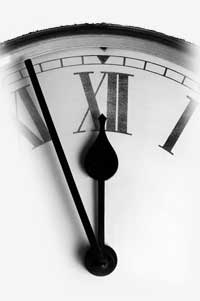
\includegraphics[width=\linewidth]{bilder/uhr}}
\parbox{.9\linewidth}{
\begin{aufzaehlung}
\item \url{www.asta.rwth-aachen.de} -- Webseiten des AStA mit aktuellen Infos und Sprechzeiten der BAf"oG-Beratung
\item \url{www.bafoeg.bmbf.de} -- Bundesministerium f�r Bildung und Forschung, Informationen und BAf"oG-Rechner
\item \url{www.studentenwerk-aachen.de} -- BAf"oG-Amt Aachen
\item \url{www.studis-online.de} und \url{www.bafoegrechner.de} -- aktuelle Infos rund ums BAf"oG
\end{aufzaehlung}}
\vspace*{1ex}

Der AStA bietet auch eine pers"onliche Beratung an. Die genauen Termine findest Du in der unten stehenden Kontaktbox oder auf unserer Webseite unter \url{www.asta.rwth-aachen.de/beratung}. Eine vorherige Terminabsprache ist nicht notwendig. Die Beratung ist kostenlos und erfolgt selbstverst"andlich vertraulich.
\end{artikel}

\end{rueckseite}
%<geschweifteKlammer>
\end{document}  

\renewcommand{\thefootnote}{\arabic{footnote}}
